% Mainfile:
%%%***++ mainfile.tex
% !arara: pdflatex: { files: [ mainfile.tex ] }
% arara: makechapters: { files:[mainfile], items: [module3], makeChapGlossaries: no}
% !arara: indent: { overwrite: on, trace: yes}
\chapter{Multiplying Polynomials}
\minitoc
\section{Special Binomial Products}
\textref{6.3}{360}%
In the previous module we examined some elementary \gls{polynomial} multiplication. We begin
this module by considering the following polynomial multiplications, all of which will
be done using the \gls{FOIL} method. In this section, we will:
\begin{enumerate}
	\item Multiply the sum and difference of 2 terms
	\item Find the square of a \gls{binomial} sum.
	\item Find the square of a binomial difference
\end{enumerate} 

\subsection{The FOIL method}
We will often be finding the product of 2 binomials, such as
\[
	(x-2)(x+3)
\]
so it will be useful to develop a solid place from which to start. There is a well known
acronym that can help us, which is {\bfseries FOIL}. We describe it as follows
\begin{description}
	\item Multiply the  {\color{red}F}irst terms from each binomial, then 
	\item	Multiply the  {\color{green}O}utside terms, then                
	\item	Multiply the  {\color{brown}I}nside terms, and finally          
	\item	Multiply the  {\color{blue}L}ast terms                          
\end{description}
The FOIL method distributes the 1st term, and then distributes the 2nd. In the above example the 
components of the FOIL are
\begin{itemize}
	\item {\color{red}F}: the {\em first} terms multiplied together are $x\cdot x = x^2$
	\item {\color{green}O}: the {\em outside} terms multiplied together are $x\cdot 3 = 3x$
	\item {\color{brown}I}: the {\em inside} terms are $-2\cdot x = -2x$
	\item {\color{blue}L}: the {\em last} terms are $-2(3)=-6$
\end{itemize} 
We combine all of this information as follows
\begin{align*}
	(x-2)(x+3) & =		x^2+3x-2x-6 \\
	           & =		x^2+x-6     
\end{align*} 	

\begin{myexample}
Use the FOIL method to expand the following polynomial 
\[
	(3x+2)(4x+5)
\]
\end{myexample}
\begin{myProof}
	We colour code the polynomial as follows
	\begin{tightcenter}
		\begin{tabular}{lll}
			$({\color{red}3x}+2)({\color{red}4x}+2)$     & First terms {\color{red}F}   & ${\color{red}(3x)(4x)=12x^2}$ \\
			$({\color{green}3x}+2)(4x+{\color{green}5})$ & Outer terms {\color{green}O} & ${\color{green}(3x)(5)=15x}$  \\	
			$(3x+{\color{brown}2})({\color{brown}4x}+5)$ & Inner terms {\color{brown}I} & ${\color{brown}(2)(4x)=8x}$   \\	
			$(3x+{\color{blue}2})(4x+{\color{blue}{5}})$ & Last terms {\color{blue}L}   & ${\color{blue}(2)(5)=10}$     
		\end{tabular} 
	\end{tightcenter}
	More simply, we can write
	\begin{align*}
		(3x+2)(4x+5) & =		{\color{red}12x^2}+{\color{green}15x}+{\color{brown}{8x}}+{\color{blue}{10}} \\
		             & =		12x^2+23x+10                                                                 
	\end{align*} 
\end{myProof} 

\begin{myexample}
\Gls{simplify} the following.
\drillandskill
\end{myexample}
\begin{enumerate}
	\item $(x+1)(x+2)$\solution{$=x^2+3x+2$}
	\item $(x-1)(x-4)$\solution{$=x^2-5x+4$}
	\item $(2x+1)(x-5)$\solution{$=2x^2-9x-5$}
	\item $(3x-4)(x+6)$\solution{$=3x^2+14x-24$}
\end{enumerate}

\subsection{Multiplying the Sum and Difference of 2 terms}
When using the FOIL method, there are a number of special products that arise, 
for example
\[
	(a-b)(a+b)
\]
When using the FOIL method on a product of this form, which is the product of the sum of two terms with the product
of the difference of two terms, there is a useful simplification
\begin{align*}
	(a-b)(a+b) & =		a^2+ab-ba-b^2 \\
	           & =		a^2-b^2       
\end{align*} 
Notice here that the `middle' terms (the {\color{green}O}utside and the {\color{brown}I}nside terms) cancel each other out. This will 
be particularly useful in later modules when we are asked to \gls{factor} a polynomial, which involves `going the other way' from FOILing. 

\begin{myexample}\label{ex:sumdiff}
Use the FOIL method to expand the following \gls{expression}
\[
	(x-3)(x+3)
\]
\end{myexample}
\begin{myProof}
	We note first of all that this is the product of the sum and difference of two terms, so the middle terms will cancel. We will show the
	working for demonstration
	\begin{align*}
		(x-3)(x+3) & =		x^2+3x-3x-9 \\
		           & =		x^2-9       
	\end{align*} 
\end{myProof} 

\begin{myexample}
Simplify the following.
\drillandskill
\end{myexample}
\begin{enumerate}
	\item $(x+10)(x-10)$\solution{$=x^2-100$}
	\item $(x+3)(x-3)$\solution{$=x^2-9$}
	\item $(x-4)(x+4)$\solution{$=x^2-16$}
	\item $(x^4-7)(x^4+7)$\solution{$=x^8-49$}
	\item $(3x+1)(3x-1)$\solution{$=9x^2-1$}
	\item $(2x+4)(2x-4)$\solution{$=4x^2-16$}
\end{enumerate}

\subsection{The Square of a Binomial Sum}\label{sec:binsum}
Another special case of a binomial \footnote{ Remember that a {\em binomial} is simply another way of saying a polynomial with 2 terms.} 
multiplication is the square of a binomial sum, for example
\[
	(x+y)^2
\] 
Using the FOIL method on this expression, we achieve
\begin{align*}
	(x+y)^2 & =		x^2+xy+xy+y^2 \\
	        & =		x^2+2xy+y^2   
\end{align*} 
In words: The square of a binomial sum is the first term squared, plus two times the product of the terms, plus the last term squared.

\begin{myexample}
Use the FOIL method to expand the following polynomial 
\[
	(2x+5)^2
\]
\end{myexample}
\begin{myProof}
	We apply the FOIL method and obtain
	\begin{align*}
		(2x+5)^2 & =		(2x)^2+(2x)(5)+(2x)(5)+5^2 \\
		         & =		4x^2+10x+10x+25            \\
		         & =		4x^2+20x+25                
	\end{align*} 
\end{myProof} 

\begin{myexample}
Simplify the following.
\drillandskill
\end{myexample}
\begin{enumerate}
	\item $(x+1)^2$\solution{$=x^2+2x+1$} 
	\item $(x+6)^2$\solution{$=x^2+12x+36$}
	\item $(x+10)^2$\solution{$=x^2+20x+100$}
	\item $(x+7)^2$\solution{$=x^2+14x+49$}
	\item $(x^2+9)^2$\solution{$=x^4+18x^2+81$}
	\item $(2x+4)^2$\solution{$=4x^2+16x+16$}
\end{enumerate}

\subsection{The Square of a Binomial Difference}\label{sec:bindiff}
The final special case of a binomial multiplication is the square of a binomial difference, for example
\[
	(x-2)^2
\]
Using the FOIL method gives
\begin{align*}
	(x-2)^2 & =		x^2-2x-2x+4 \\
	        & =		x^2-4x+4    
\end{align*} 
In general
\[
	(x-y)^2 = x^2-2xy+y^2
\]
\begin{myexample}
Use the FOIL method to expand the following polynomial 
\[
	(4x-6)^2
\]
{}
\end{myexample}
\begin{myProof}
	On applying the FOIL procedure, we obtain
	\begin{align*}
		(4x-6)^2 & =		(4x)^2+(4x)(-6)+(4x)(-6)+(-6)^2 \\
		         & =		16x^2 - 24x - 24x +36           \\
		         & =		16x^2-48x+36                    
	\end{align*} 
\end{myProof}

\begin{myexample}
Simplify the following.
\drillandskill
\end{myexample}
\begin{enumerate}
	\item $(x-1)^2$\solution{$=x^2-2x+1$}
	\item $(x-6)^2$\solution{$=x^2-12x+36$}
	\item $(x-10)^2$\solution{$=x^2-20x+100$}
	\item $(x-7)^2$\solution{$=x^2-14x+49$}
	\item $(x^2-9)^2$\solution{$=x^4-18x^2+81$}
	\item $(2x-4)^2$\solution{$=4x^2-16x+16$}
\end{enumerate}

\subsection{Miscellaneous FOIL examples}
\begin{myexample}
Find an expression for each of the following shaded areas (diagrams not to scale).
\end{myexample}
\begin{minipage}[t]{.5\textwidth}
	\centering
	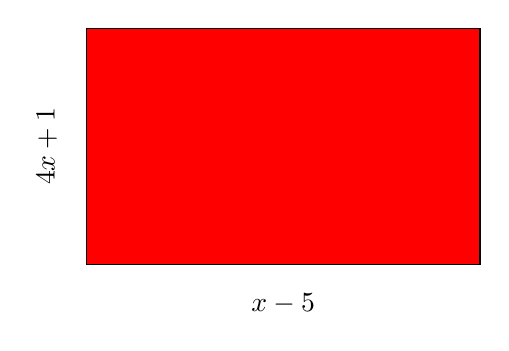
\begin{tikzpicture}
		\draw[fill=red] (0,0) rectangle (5,3);
		\draw (-.5,1.5) node[rotate=90] {$4x+1$};
		\draw (2.5,-.5) node {$x-5$};
	\end{tikzpicture}
	\begin{align*}
		area & =  (4x+1)(x-5) \\
		     & = 4x^2-19x-5   
	\end{align*} 
\end{minipage}
\begin{minipage}[t]{.5\textwidth}
	\centering
	\begin{tikzpicture}
		\draw[fill=blue] (0,0) rectangle (5,3);
		\draw (-.5,1.5) node[rotate=90] {$4x+1$};
		\draw (2.5,-.5) node {$x-5$};
		\filldraw [white,draw=black] (3,1.5) circle (1);
		\draw (3,1.5)--(4,1.5) node (myradius){};
		\node[node distance=0cm,above left = of myradius] {$x$};
	\end{tikzpicture}
	\begin{align*}
		area & =  (4x+1)(x-5)-\pi x^2 \\
		     & = 4x^2-19x-5 - \pi x^2 \\
		     & = (4-\pi)x^2-19x-5     
	\end{align*} 
\end{minipage}

\begin{minipage}[t]{.5\textwidth}
	\centering
	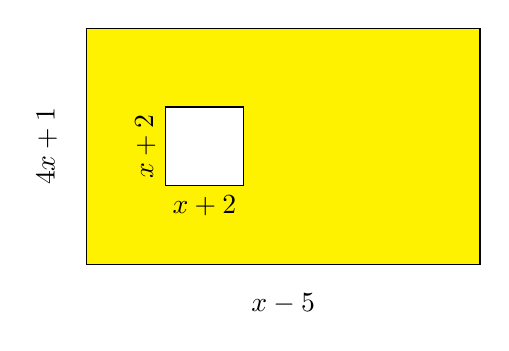
\begin{tikzpicture}
		\draw[fill=yellow] (0,0) rectangle (5,3);
		\draw[fill=white] (1,1) rectangle (2,2);
		\draw (-.5,1.5) node[rotate=90] {$4x+1$};
		\draw (2.5,-.5) node {$x-5$};
		\draw (1.5,.75) node {$x+2$};
		\draw (.75,1.5) node[rotate=90] {$x+2$};
	\end{tikzpicture}
	\begin{align*}
		area & =  (4x+1)(x-5)-(x+2)(x+2) \\
		     & = 4x^2-19x-5 - (x^2+4x+4) \\
		     & = 3x^2-23x-9              
	\end{align*} 
\end{minipage}
\begin{minipage}[t]{.5\textwidth}
	\centering
	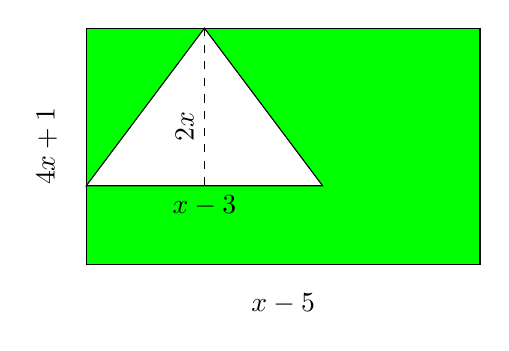
\begin{tikzpicture}
		\draw[fill=green] (0,0) rectangle (5,3);
		\draw (-.5,1.5) node[rotate=90] {$4x+1$};
		\draw (2.5,-.5) node {$x-5$};
		\draw[fill=white] (0,1)--(3,1)--(1.5,3)--cycle;
		\draw[dashed] (1.5,1)--(1.5,3);
		\draw (1.25,1.75) node[rotate=90] {$2x$};
		\draw (1.5,0.75) node {$x-3$};
	\end{tikzpicture}
	\begin{align*}
		area & =  (4x+1)(x-5)- \frac{1}{2}(2x)(x-3) \\
		     & = 4x^2-19x-5 - (x^2-3x)              \\
		     & = 3x^2-16x-5                         
	\end{align*} 
\end{minipage}

\begin{myexample}
Here are some miscellaneous short cut FOIL examples.
\drillandskill
\end{myexample}
\begin{myProof}
	Can you spot  which short cut to use? If not, don't worry, just FOIL!
				
	\begin{multicols}{2}
		\begin{enumerate}
			\item $(x+1)^2$\solution{$=x^2+2x+1$}
			\item $(x+2)^2$\solution{$=x^2+4x+4$}
			\item $(x+5)^2$\solution{$=x^2+10x+25$}
			\item $(x-1)^2$\solution{$=x^2-2x+1$}
			\item $(2x+1)^2$\solution{$=4x^2+4x+1$}
			\item $(2x-1)^2$\solution{$=4x^2-4x+1$}
			\item $(x-3)^2$\solution{$=x^2-6x+9$}
			\item $(2x+4)^2$\solution{$=4x^2+16x+16$}
			\item $(3x+2)^2$\solution{$=9x^2+12x+4$}
			\item $(2-x)^2$\solution{$=x^2-4x+4$}
			\item $(3-x)^2$\solution{$=x^2-6x+9$}
			\item $(2+x)^2$\solution{$=x^2+4x+4$}
			\item $(2-3x)^2$\solution{$=9x^2-12x+4$}
			\item $(2x+5)^2$\solution{$=4x^2+20x+25$}
			\item $(x-1)(x+1)$\solution{$=x^2-1$}
			\item $(x-2)(x+2)$\solution{$=x^2-4$}
			\item $(x+3)(x-3)$\solution{$=x^2-9$}
			\item $(2x-1)(2x+1)$\solution{$=4x^2-1$}
			\item $(1-x)(1+x)$\solution{$=1-x^2$}
			\item $(x+2)(x-2)$\solution{$=x^2-4$}
			\item $(x-5)(x+5)$\solution{$=x^2-25$}
			\item $(3x+3)(3x-3)$\solution{$=9x^2-9$}
		\end{enumerate}
	\end{multicols}
\end{myProof} 

\subsection{The cube of a binomial sum}
We can find the \emph{cube} of a binomial sum by using the FOIL technique combined 
with polynomial multiplication.
\begin{myexample}
Expand the following polynomial by using polynomial multiplication
\[
	(x+y)^3
\]
\end{myexample}
\begin{myProof}
$
\begin{aligned}[t]
(x+y)^3 & = (x+y)(x+y)^2\\
& = (x+y)(x^2+2xy+y^2)\\
& = x^3+2x^2y+xy^2 + yx^2 + 2xy^2 + y^3\\
& = x^3 + 3x^2y + 3 xy^2 + y^3
\end{aligned}
$
\end{myProof}
\begin{myexample}
Here are some miscellaneous short-cut cube examples.
\drillandskill
\end{myexample}
\begin{myProof}				
		\begin{enumerate}
			\item $(x+1)^3$\solution{$=x^3+3x^2+3x+1$}
			\item $(x+2)^3$\solution{$=x^3+6x^2+12x+8$}
			\item $(2x+3)^3$\solution{$=8x^3+36x^2+54x+27$}
			\item $(3x+2y)^3$\solution{$=27x^3+54x^2y+36x*y^2+8y^3$}
		\end{enumerate}
\end{myProof} 

\subsection{The cube of a binomial difference}
We can find the \emph{cube} of a binomial difference by using the FOIL technique combined 
with polynomial multiplication- this is very similar to the technique used for the 
cube of binomial sum.
\begin{myexample}
Expand the following polynomial by using polynomial multiplication
\[
	(x-y)^3
\]
\end{myexample}
\begin{myProof}
$
\begin{aligned}[t]
(x-y)^3 & = (x-y)(x-y)^2\\
& = (x-y)(x^2-2xy+y^2)\\
& = x^3-2x^2y+xy^2 - yx^2 + 2xy^2 - y^3\\
& = x^3 -3x^2y + 3 xy^2 - y^3
\end{aligned}
$
\end{myProof}
\begin{myexample}
Here are some miscellaneous short-cut cube examples.
\drillandskill
\end{myexample}
\begin{myProof}				
		\begin{enumerate}
			\item $(x-1)^3$\solution{$=x^3-3x^2+3x-1$}
			\item $(x+2)^3$\solution{$=x^3-6x^2+12x-8$}
			\item $(2x+3)^3$\solution{$=8x^3-36x^2+54x-27$}
			\item $(3x+2y)^3$\solution{$=27x^3-54x^2y+36x*y^2-8y^3$}
		\end{enumerate}
\end{myProof} 




\subsection{An application}
The following is an application of our work in polynomials.
\begin{myexample}\label{ex:fallingobject}
Consider the \gls{equation} of motion for an object tossed straight up into the air (projected vertically), 
or dropped (falling)
\begin{equation}\label{eq:objectfalling}
	s = -\frac{1}{2}gt^2+v_0t+s_0
\end{equation}
Note the following:
\begin{itemize}
	\item $s$ is vertical position (height above ground) of the tossed object in feet (ft)
	\item $g$ is the acceleration due to gravity (and we will assume $g=32$)
	\item $t$ is time in seconds that the object has been in motion (seconds)
	\item $v_0$ is the initial speed (or velocity) of the object in ft/sec
	\item $s_0$ is the initial position at time $t=0$
\end{itemize} 
Find the height of ball after
\begin{multicols}{3}
	\begin{enumerate}
		\item $2$ seconds
		\item $4$ seconds
		\item $6$ seconds
	\end{enumerate} 
\end{multicols} 
\end{myexample}
\begin{myProof}
	Before we begin this example, we first need to rewrite \cref{eq:objectfalling} using
	the given information. It becomes
	\[
		s = -16t^2+80t+96
	\]
	To find the height of the object at each of the specified times, we will simply replace $t$ by 2, 4, and 6 seconds in turn.
	\begin{enumerate}
		\item After 2 seconds, the height of the object (in feet) is
		\[
			-16(2^2)+80(-2)+96 = 192
		\]
		\item After 4 seconds, the height of the object (in feet) is
		\[
			-16(4^2)+80(4)+96=160
		\]
		\item After 6 seconds, the height of the object (in feet) is
		\[
			-16(6^2)+80(6)+96=0
		\]
	\end{enumerate} 
	We clearly see that as time increase, the height of the object is decreasing. In fact, after
	6 seconds the ball is at a height of 0ft above the ground- in other words it has hit the ground
	at this time.
				
	\Cref{fig:fallingobject2} shows a visual representation of the height of the object thrown in 
	the example considered so far.
				
	\begin{figure}[!h]
		\centering
		\begin{tikzpicture}
			\begin{axis}[
					framed,
					axis line style={->},
					xmin=-1,xmax=10,
					ymin=-20,ymax=200,
					xlabel={$t$},
					ylabel={$s$},
					xtick={0,2,...,8},
					ytick={0,20,...,180},
					grid=major,
					scatter/classes={a={mark=*,draw=violet,fill=violet,scale=1},%
						b={mark=*,draw=red,fill=red,scale=1},
						c={mark=*,draw=black,fill=black,scale=1},
						d={scale=0}}
				]
				\addplot[red]expression[domain=0:6,samples=100]{-16*x^2+80*x+96};
			\end{axis}
		\end{tikzpicture}
		\caption{A falling object}
		\label{fig:fallingobject2}
	\end{figure}
	\FloatBarrier
				
	The horizontal axis represents the object's time in seconds. The vertical axis represents
	the object's height above the ground.
	\begin{itemize}
		\item During which time period is the object increasing in height? \\
		We see that the height is increasing from $t=0$ to approximately
		$t=2.5$ seconds.
		\item During which time period is the object decreasing in height?\\
		We see that the height is decreasing from approximately $t=2.5$ seconds
		to $t=6$ seconds.
		\item After how much time does the object strike the ground?\\
		The object strikes the ground when the graph cuts the horizontal
		axis, which happens when $t=6$.
		\item After how many seconds does the object reach its maximum height? Give an
		approximation of this height.\\
		The maximum value of the height (which we will later discuss as the {\em \gls{vertex}} of
		the graph) occurs when $t \approx 2.5$, and looking at the vertical scale, we see
		that the maximum height is approximately 195ft.
	\end{itemize} 
\end{myProof}

\section{Polynomials in several variables}
\textref{6.4}{368}%
We have so far seen some elementary polynomial operations, using the FOIL 
method to expand special products involving binomials. In this section we will build 
on this, and discuss polynomials of more than one \gls{variable}.

\subsection{Evaluate polynomials in several variables}
We will introduce this in terms of a real world example.

\begin{myexample}\label{ex:storageshed}
The storage shed given below has a volume of
\[
	V= 2x^2y+ \frac{1}{2}\pi x^2 y
\]
\begin{figure}[!h]
	\centering
	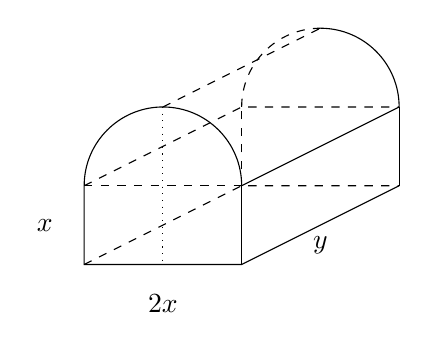
\begin{tikzpicture}
		% foreground stuff
		\draw (0,1)--(0,0)--(2,0)--(4,1);
		\draw (2,1)--(4,2);
		\draw (2,0)--(2,1);
		\draw (4,1)--(4,2);
		\draw (2,1) arc (0:180:1);
		\draw (4,2) arc (0:90:1);
		% background stuff
		\draw[dashed] (2,2) arc (180:90:1);
		\draw[dashed] (0,1)--(2,2)--(4,2);
		\draw[dashed] (0,0)--(2,1)--(4,1);
		\draw[dashed] (2,1)--(2,2);
		\draw[dashed] (1,2)--(3,3);
		\draw[dashed] (0,1)--(2,1);
		\draw[dotted] (1,2)--(1,0);
		% labels
		\node at (1,-.5) {$2x$};
		\node at (-.5,.5) {$x$};
		\node at (3,.25) {$y$};
	\end{tikzpicture}
	\caption{A storage shed}
\end{figure}
\FloatBarrier
			
The small business that owns this storage shed tells you that the variables have the following 
values
\[
	x = 13, y = 27
\]
where both measurements are given in ft. 
			
Find the volume of the storage shed that has these
dimensions.
\end{myexample}
\begin{myProof}
	To find the required volume, we use our original expression for $V$, and replace each occurrence of $x$
	with 13, and each occurrence of $y$ with 27. This gives
	\begin{align*}
		V & =		2(13)^2\cdot 27 + \frac{1}{2}\pi (13)^2	\cdot 27 \\
		  & =		2(169)(27)+\frac{1}{2}\pi(169)(27)               \\
		  & =		9126+2281.5\pi                                   
	\end{align*} Note that this answer is {\em exact}, as we have not had to approximate any of the values
	involved. For practical purposes, we may need an approximation, so we use the $\pi$ key on our calculators,
	and obtain
	\[
		V \approx 16293.54 ft^3
	\]
	{\bfseries Important note}: Notice how we have used the $\approx$ symbol to represent
	`approximately equal to'; it is very important to distinguish between this and the regular $=$ symbol.
				
\end{myProof} 

The steps that we followed in \cref{ex:storageshed} can be summarized as follows:
\begin{itemize}
	\item Substitute the given value for each variable
	\item Perform the resulting computation, being careful to use the order of operations - notice how we evaluated
	the term with the exponent before we did any further multiplication.
\end{itemize} 

\subsection{The vocabulary of polynomials in two variables}
This carries across very naturally from our work in one variable polynomials. In general, a polynomial in two variables
$x$ and $y$

\begin{itemize}
	\item contains the sum of one or more monomials which have the form
	\[
		a x^n y^m
	\]
	\item here $a$ is the \gls{coefficient}
	\item and the \gls{degree} of this term is $n+m$
\end{itemize} 

\begin{myexample}
Find the degree of the following polynomials
\begin{multicols}{2}
	\begin{enumerate}
		\item $x^2y^3$
		\item $xy^2z^3$
	\end{enumerate} 
\end{multicols}
\end{myexample}
\begin{myProof}
	\begin{enumerate}
		\item The power of $x$ is 2, and power of $y$ is 3, so the degree of this term is $2+3=5$
		\item The power of $x$ is 1, the power of $y$ is 2, and the power of $z$ is 3, so the degree of this term
		is $1+2+3=6$
	\end{enumerate}	
\end{myProof} 


\subsection{Adding and subtract polynomials in several variables}
Adding and subtracting polynomials in several variables applies the principles that we learnt for adding and subtracting those
with just one variable
\begin{itemize}
	\item {\em Addition}: combine like terms
	\item {\em Subtraction}: distribute subtraction signs appropriately, and then add
\end{itemize} 

\subsection{Multiplying monomials (in $x$ and $y$)}
To multiply monomials with more than one variable we multiply the coefficients, and add the exponents on variables that have the same base.

\begin{myexample}
Multiply the following
\[
	(7x^2y)(5x^3y^2)
\]
\end{myexample}
\begin{myProof}
	As described above, we multiply the 7 and the 5, and combine the $x$ and $y$ terms using the properties
	of exponents discussed previously.
	\begin{align*}
		(7x^2y)(5x^3y^2) & =		35x^2x^3yy^2 \\
		                 & =		35x^5y^3     
	\end{align*} 
\end{myProof} 

\subsection{Multiplying a \gls{monomial} with a polynomial}
This follows the same method as that of the one variable case: we distribute the monomial through the polynomial, 
and then multiply as detailed in the previous example.

\begin{myexample}
Simplify the following expression
\[
	3x^2y(2x^3+5x+1)
\]
\end{myexample}
\begin{myProof}
	We follow the procedure outlined above
	\begin{align*}
		3x^2y(2x^3+5x+1) & =		3x^2y(2x^3)+3x^2y(5x)+3x^2y(1) \\
		                 & =		3(2)x^2x^3y+3(5)x^2xy+3x^2y    \\
		                 & =		6x^5y+15x^3y+3x^2y             
	\end{align*} 
\end{myProof}

\begin{myexample}
Simplify the following.
\drillandskill
\end{myexample}

\begin{enumerate}
	\item $2y^2(x^2y^3+xy+x)$\solution{$=2x^2y^5+2xy^3+2xy^2$}
	\item $-3xy(x^2+y^2+xy)$\solution{$=-3x^3y-3xy^3-3x^2y^2$}
	\item $-4x(x+y)(x-y)$\solution{$=-4x^3+4xy^2$}
	\item $x^2y^5(x^2+y^2)$\solution{$=x^4y^5+x^2y^7$}
\end{enumerate}


\subsection{Multiplying binomials with binomials }
We use the same FOIL procedure that we have used previously.

\begin{myexample}
Multiply the following
\begin{multicols}{2}
	\begin{enumerate}
		\item $(5x-3y)(5x+3y)$
		\item $(6x+4y)^2$
		\item $(9x-3y)^2$
		\item $(a^2+3b)(5a^2-4b)$
	\end{enumerate} 
\end{multicols}
\end{myexample}

\begin{myProof}
	\begin{enumerate}
		\item Notice that this is the multiplication of the sum and difference of 2 terms (see \cref{ex:sumdiff})
		\begin{align*}
			(5x-3y)(5x+3y) & =		(5x)^2-(3y)^2 \\
			               & =		25x^2-9y^2    
		\end{align*}		 
		\item Notice that this is the square of a binomial sum (see \cref{sec:binsum})
		\begin{align*}
			(6x+4y)^2 & =		(6x)^2+2(6)(4)xy+(4y)^2 \\
			          & =		36x^2+48xy+16y^2        
		\end{align*} 
		\item Notice that this is the square of a binomial difference (see \cref{sec:bindiff})
		\begin{align*}
			(9x-3y)^2 & =		(9x)^2-2(9)(3)xy+(3y)^2 \\
			          & =		81x^2-54xy+9y^2         
		\end{align*} 
		\item This does not fall into one of the special cases that we have discussed, so we simply FOIL it
		\begin{align*}
			(a^2+3b)(5a^2-4b) & =		5a^4-4a^2b+15ba^2-12b^2 \\
			                  & =		5a^4+11a^2b-12b^2       
		\end{align*} 
	\end{enumerate} 
\end{myProof} 

\begin{myexample}
Simplify the following.
\drillandskill
\end{myexample}
\begin{enumerate}
	\item $(x+y)^2$\solution{$=x^2+2xy+y^2$}
	\item $(x-y)^2$\solution{$=x^2-2xy+y^2$}
	\item $(x-y)(x+y)$\solution{$=x^2-y^2$}
	\item $(x+y)(x-y)$\solution{$=x^2-y^2$}
\end{enumerate}

\begin{myexample}
Find an expression for each of the following shaded areas (diagrams not to scale).
\end{myexample}

\begin{minipage}[t]{.5\textwidth}
	\centering
	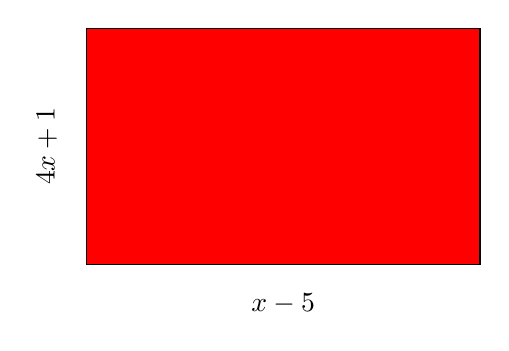
\begin{tikzpicture}
		\draw[fill=red] (0,0) rectangle (5,3);
		\draw (-.5,1.5) node[rotate=90] {$4x+1$};
		\draw (2.5,-.5) node {$x-5$};
	\end{tikzpicture}
	{$area=4x^2-19x-5$}
\end{minipage}
\begin{minipage}[t]{.5\textwidth}
	\centering
	\begin{tikzpicture}
		\draw[fill=blue] (0,0) rectangle (5,3);
		\draw (-.5,1.5) node[rotate=90] {$4x+1$};
		\draw (2.5,-.5) node {$x-5$};
		\filldraw [white,draw=black] (3,1.5) circle (1);
		\draw (3,1.5)--(4,1.5) node (myradius){};
		\node[node distance=0cm,above left = of myradius] {$y$};
	\end{tikzpicture}
	{$area=4x^2-\pi y^2-19x-5$}
\end{minipage}

\begin{minipage}[t]{.5\textwidth}
	\centering
	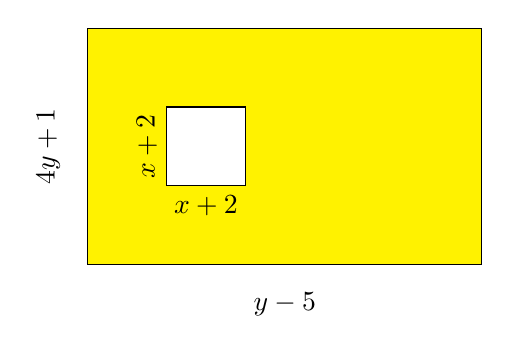
\begin{tikzpicture}
		\draw[fill=yellow] (0,0) rectangle (5,3);
		\draw[fill=white] (1,1) rectangle (2,2);
		\draw (-.5,1.5) node[rotate=90] {$4y+1$};
		\draw (2.5,-.5) node {$y-5$};
		\draw (1.5,.75) node {$x+2$};
		\draw (.75,1.5) node[rotate=90] {$x+2$};
	\end{tikzpicture}
	{$area=4y^2-x^2-19y-4x-9$}
\end{minipage}
\begin{minipage}[t]{.5\textwidth}
	\centering
	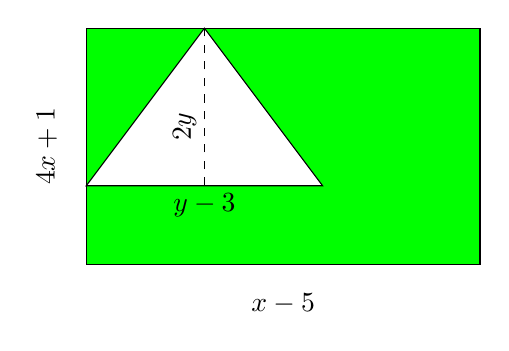
\begin{tikzpicture}
		\draw[fill=green] (0,0) rectangle (5,3);
		\draw (-.5,1.5) node[rotate=90] {$4x+1$};
		\draw (2.5,-.5) node {$x-5$};
		\draw[fill=white] (0,1)--(3,1)--(1.5,3)--cycle;
		\draw[dashed] (1.5,1)--(1.5,3);
		\draw (1.25,1.75) node[rotate=90] {$2y$};
		\draw (1.5,0.75) node {$y-3$};
	\end{tikzpicture}
	{$area=4x^2-y^2-19x+3y-5$}
\end{minipage}

\begin{minipage}[t]{.5\textwidth}
	\centering
	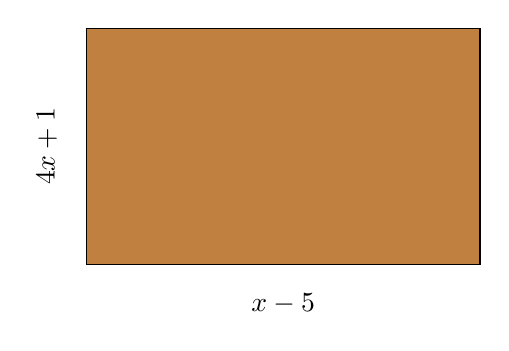
\begin{tikzpicture}
		\draw[fill=brown] (0,0) rectangle (5,3);
		\draw (-.5,1.5) node[rotate=90] {$4x+1$};
		\draw (2.5,-.5) node {$x-5$};
	\end{tikzpicture}
	{$area=3xy-15y+x-5$}
\end{minipage}
\begin{minipage}[t]{.5\textwidth}
	\centering
	\begin{tikzpicture}
		\draw[fill=purple] (0,0) rectangle (5,3);
		\draw (-.5,1.5) node[rotate=90] {$4x+1$};
		\draw (2.5,-.5) node {$x-5$};
		\filldraw [white,draw=black] (3,1.5) circle (1);
		\draw (3,1.5)--(4,1.5) node (myradius){};
		\node[node distance=0cm,above left = of myradius] {$y$};
	\end{tikzpicture}
	{$area=4xy-\pi x^2-20x+y-5$}
\end{minipage}
